\section{Durchführung}
\label{sec:Durchführung}

Der Versuchsaufbau beinhaltet aus einem Ultraschallechoskop,
Ultraschallsonden verschiedener Frequenzen, einem Computer
zur Datenaufnahme und einem Kippschalter, der zwischen
Durchschallung- und Impuls-Echo-Verfahren wechselt. \\

Zuerst wird ein Acrylblock (s. Abbildung \ref{fig:block}) mit dem A-Scan untersucht.
Die Abmessungen des Blockes werden mithilfe einer 
Schieblehre, darauf die Lage der Bohrungen mit dem
Impuls-Echo-Verfahren, und deren Tiefe mit dem A-Scan
aus verschiedenen Winkeln bestimmt. Angewendet wird das Impuls-Echo-Verfahren 
mit jeweils verschieden $\SI{1}{\mega\hertz}$-, $\SI{2}{\mega\hertz}$- und 
$\SI{4}{\mega\hertz}$-Sonden, deren Signale am Computer ausgewertet werden.
Dazu wird die Laufzeit mittels Cursoren als Differenz zwischen den aufgenommenen Peaks gemessen.
Als Koppelmittel wird destilliertes Wasser verwendet. \\

\begin{figure} [H]
    \centering
    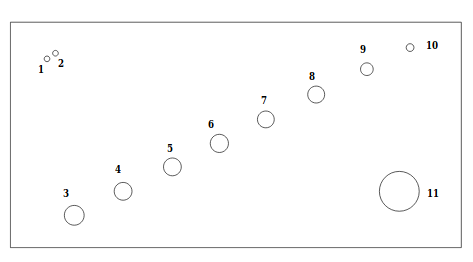
\includegraphics[scale=0.5]{content/bild1.png}
    \caption{Querschnitt des zu vermessenden Acrylblocks mit nummerierten Störstellen [1]}
    \label{fig:block}
  \end{figure}

Das Auflösungsvermögen wird durch die Messung zweier
nebeneinanderliegender Bohrungen untersucht.\\

Zudem wird der Acrylblock mit dem B-Scan auf zwei gegenüberliegenden Seiten,
diesmal aber nur mit
der $\SI{2}{\mega\hertz}$-Sonde untersucht. Dabei ist
auf eine konstante Geschwindigkeit der Sondenbewegung zu achten.
Auch hier wird als Koppelmittel destilliertes Wasser verwendet.\\

Zuletzt wird an einem Herzmodell der TM-Scan mit der $\SI{2}{\mega\hertz}$-Sonde durchgeführt.
Dieses wird zu einem Drittel mit Wasser gefüllt und ein
A-Scan der Echolaufzeit durchgeführt.
Dabei soll das Herzvolumen durch Luftdruckänderung an einer
Membran vergrößert und verkleinert werden
und der menschliche Herzschlag simuliert werden.

